\iffalse
This file is protected by Copyright. Please refer to the COPYRIGHT file
distributed with this source distribution.

This file is part of OpenCPI <http://www.opencpi.org>

OpenCPI is free software: you can redistribute it and/or modify it under the
terms of the GNU Lesser General Public License as published by the Free Software
Foundation, either version 3 of the License, or (at your option) any later
version.

OpenCPI is distributed in the hope that it will be useful, but WITHOUT ANY
WARRANTY; without even the implied warranty of MERCHANTABILITY or FITNESS FOR A
PARTICULAR PURPOSE. See the GNU Lesser General Public License for more details.

You should have received a copy of the GNU Lesser General Public License along
with this program. If not, see <http://www.gnu.org/licenses/>.
\fi
%----------------------------------------------------------------------------------------
% Update the docTitle and docVersion per document
%----------------------------------------------------------------------------------------
\def\docTitle{Vivado Usage Guide}
\def\docVersion{1.4}
%----------------------------------------------------------------------------------------
\documentclass{article}
\iffalse
This file is protected by Copyright. Please refer to the COPYRIGHT file
distributed with this source distribution.

This file is part of OpenCPI <http://www.opencpi.org>

OpenCPI is free software: you can redistribute it and/or modify it under the
terms of the GNU Lesser General Public License as published by the Free Software
Foundation, either version 3 of the License, or (at your option) any later
version.

OpenCPI is distributed in the hope that it will be useful, but WITHOUT ANY
WARRANTY; without even the implied warranty of MERCHANTABILITY or FITNESS FOR A
PARTICULAR PURPOSE. See the GNU Lesser General Public License for more details.

You should have received a copy of the GNU Lesser General Public License along
with this program. If not, see <http://www.gnu.org/licenses/>.
\fi
\author{} % Force author to be blank
%----------------------------------------------------------------------------------------
% Paper size, orientation and margins
%----------------------------------------------------------------------------------------
\usepackage{geometry}
\geometry{
        letterpaper, % paper type
        portrait,    % text direction
        left=.75in,  % left margin
        top=.75in,   % top margin
        right=.75in, % right margin
        bottom=.75in % bottom margin
 }
%----------------------------------------------------------------------------------------
% Header/Footer
%----------------------------------------------------------------------------------------
\usepackage{fancyhdr} \pagestyle{fancy} % required for fancy headers
\renewcommand{\headrulewidth}{0.5pt}
\renewcommand{\footrulewidth}{0.5pt}
\rhead{\small{ANGRYVIPER Team}}
% \rfoot{\thepage}
%----------------------------------------------------------------------------------------
% Appendix packages
%----------------------------------------------------------------------------------------
\usepackage[toc,page]{appendix}
%----------------------------------------------------------------------------------------
% Defined Commands & Renamed Commands
%----------------------------------------------------------------------------------------
\renewcommand{\contentsname}{Table of Contents}
\renewcommand{\listfigurename}{List of Figures}
\renewcommand{\listtablename}{List of Tables}
%----------------------------------------------------------------------------------------
% Various packages
%----------------------------------------------------------------------------------------
\usepackage[usenames,dvipsnames]{xcolor} % for color names see https://en.wikibooks.org/wiki/LaTeX/Colors
\usepackage{hyperref}  % for linking urls and lists
\usepackage{graphicx}  % for including pictures by file
\usepackage{listings}  % for coding language styles
\usepackage{rotating}  % for sideways table
\usepackage{pifont}    % for sideways table
\usepackage{pdflscape} % for landscape view
\usepackage{subfig}
\usepackage{xstring}
\uchyph=0 % Never hyphenate acronyms like RCC (I think this overrides ANGRYVIPER above)
\renewcommand\_{\textunderscore\allowbreak} % Allow words to break/newline on underscores
%----------------------------------------------------------------------------------------
% Table packages
%----------------------------------------------------------------------------------------
\usepackage{longtable} % for long possibly multi-page tables
\usepackage{tabularx} % c=center,l=left,r=right,X=fill
% These define tabularx columns "C" and "R" to match "X" but center/right aligned
\newcolumntype{C}{>{\centering\arraybackslash}X}
\newcolumntype{R}{>{\raggedleft\arraybackslash}X}
\usepackage{float}
\floatstyle{plaintop}
\usepackage[tableposition=top]{caption}
\newcolumntype{P}[1]{>{\centering\arraybackslash}p{#1}}
\newcolumntype{M}[1]{>{\centering\arraybackslash}m{#1}}
%----------------------------------------------------------------------------------------
% Block Diagram / FSM Drawings
%----------------------------------------------------------------------------------------
\usepackage{tikz}
\usetikzlibrary{shapes,arrows,fit,positioning}
\usetikzlibrary{automata} % used for the fsm
%----------------------------------------------------------------------------------------
% Colors Used
%----------------------------------------------------------------------------------------
\usepackage{colortbl}
\definecolor{blue}{rgb}{.7,.8,.9}
\definecolor{ceruleanblue}{rgb}{0.16, 0.32, 0.75}
\definecolor{drkgreen}{rgb}{0,0.6,0}
\definecolor{deepmagenta}{rgb}{0.8, 0.0, 0.8}
\definecolor{cyan}{rgb}{0.0,0.6,0.6}
\definecolor{maroon}{rgb}{0.5,0,0}
%----------------------------------------------------------------------------------------
% VHDL Coding Language Style
% modified from: http://latex-community.org/forum/viewtopic.php?f=44&t=22076
%----------------------------------------------------------------------------------------
\lstdefinelanguage{VHDL}
{
        basicstyle=\ttfamily\footnotesize,
        columns=fullflexible,keepspaces,      % https://tex.stackexchange.com/a/46695/87531
        keywordstyle=\color{ceruleanblue},
        commentstyle=\color{drkgreen},
        morekeywords={
    library,use,all,entity,is,port,in,out,end,architecture,of,
    begin,and, signal, when, if, else, process, end,
        },
        morecomment=[l]--
}
%----------------------------------------------------------------------------------------
% XML Coding Language Style
% modified from: http://tex.stackexchange.com/questions/10255/xml-syntax-highlighting
%----------------------------------------------------------------------------------------
\lstdefinelanguage{XML}
{
        basicstyle=\ttfamily\footnotesize,
        columns=fullflexible,keepspaces,
        morestring=[s]{"}{"},
        morecomment=[s]{!--}{--},
        commentstyle=\color{drkgreen},
        moredelim=[s][\color{black}]{>}{<},
        moredelim=[s][\color{cyan}]{\ }{=},
        stringstyle=\color{maroon},
        identifierstyle=\color{ceruleanblue}
}
%----------------------------------------------------------------------------------------
% DIFF Coding Language Style
% modified from http://tex.stackexchange.com/questions/50176/highlighting-a-diff-file
%----------------------------------------------------------------------------------------
\lstdefinelanguage{diff}
{
        basicstyle=\ttfamily\footnotesize,
        columns=fullflexible,keepspaces,
        breaklines=true,                                % wrap text
        morecomment=[f][\color{ceruleanblue}]{@@},      % group identifier
        morecomment=[f][\color{red}]-,                  % deleted lines
        morecomment=[f][\color{drkgreen}]+,             % added lines
        morecomment=[f][\color{deepmagenta}]{---},      % Diff header lines (must appear after +,-)
        morecomment=[f][\color{deepmagenta}]{+++},
}
%----------------------------------------------------------------------------------------
% Python Coding Language Style
% modified from
%----------------------------------------------------------------------------------------
\lstdefinelanguage{python}
{
        basicstyle=\ttfamily\footnotesize,
        columns=fullflexible,keepspaces,
        keywordstyle=\color{ceruleanblue},
        commentstyle=\color{drkgreen},
        stringstyle=\color{orange},
        morekeywords={
    print, if, sys, len, from, import, as, open,close, def, main, for, else, write, read, range,
        },
        comment=[l]{\#}
}
%----------------------------------------------------------------------------------------
% Fontsize Notes in order from smallest to largest
%----------------------------------------------------------------------------------------
%    \tiny
%    \scriptsize
%    \footnotesize
%    \small
%    \normalsize
%    \large
%    \Large
%    \LARGE
%    \huge
%    \Huge

\date{Version \docVersion} % Force date to be blank and override date with version
\title{\docTitle}
\lhead{\small{\docTitle}}
\usepackage{enumitem}
%----------------------------------------------------------------------------------------
\begin{document}
\maketitle
\thispagestyle{fancy}
\newpage
\begin{center}
  \textit{\textbf{Revision History}}
  \begin{table}[H]
    \begin{tabularx}{\textwidth}{|c|X|l|}
      \hline
      \rowcolor{blue}
      \textbf{Revision} & \textbf{Description of Change} & \textbf{Date} \\
      \hline
      v1.2 & Initial creation for Release 1.2 & 8/2017 \\
      \hline
      v1.3 & Update for Release 1.4 & 9/2018 \\
      \hline
    \end{tabularx}
  \end{table}

\end{center}
\newpage

\tableofcontents

\newpage

\section{References}

	This document assumes a basic understanding of the Linux command line (or ``shell'') environment. A working knowledge of OpenCPI is required for understanding what vendor tools are necessary to perform various OpenCPI operations. However, no OpenCPI knowledge is required to perform the toolset installation and configuration herein. The reference(s) in Table \ref{table:references} can be used as an overview of OpenCPI and may prove useful.
\def\refcapbottom{}
\iffalse
This file is protected by Copyright. Please refer to the COPYRIGHT file
distributed with this source distribution.

This file is part of OpenCPI <http://www.opencpi.org>

OpenCPI is free software: you can redistribute it and/or modify it under the
terms of the GNU Lesser General Public License as published by the Free Software
Foundation, either version 3 of the License, or (at your option) any later
version.

OpenCPI is distributed in the hope that it will be useful, but WITHOUT ANY
WARRANTY; without even the implied warranty of MERCHANTABILITY or FITNESS FOR A
PARTICULAR PURPOSE. See the GNU Lesser General Public License for more details.

You should have received a copy of the GNU Lesser General Public License along
with this program. If not, see <http://www.gnu.org/licenses/>.
\fi

% This snippet creates the "References" table labeled "table:references"
% It creates three columns: Name, Publisher, Link and then inserts default documents
%
% To skip these defaults, define macros named
% refskipgs to skip "Getting Started"
% refskipig to skip "Installation Guide"
% refskipac to skip "Acronyms and Definitions"
% refskipocpiov to skip "OpenCPI Overview"
%
% See RPM_Installation_Guide.tex for examples
%
% After the defaults, it optionally inserts the "myreferences" macro that
% you defined elsewhere (you put hlines above all lines)
%
% If you want the \caption on the bottom, define "refcapbottom"
\begin{center}
\renewcommand*\footnoterule{} % Remove separator line from footnote
\renewcommand{\thempfootnote}{\arabic{mpfootnote}} % Use Arabic numbers (or can't reuse)
\begin{minipage}{0.9\textwidth}
  \begin{table}[H]
\ifx\refcapbottom\undefined
  \caption {References}
  \label{table:references}
\fi
  \begin{tabularx}{\textwidth}{|C|C|}
    \hline
    \rowcolor{blue}
    \textbf{Title} & \textbf{Link} \\
\ifx\refskipocpiov\undefined
    \hline
    OpenCPI Overview & \githubio{Overview.pdf} \\
\fi
\ifx\refskipac\undefined
    \hline
    Acronyms and Definitions & \githubio{Acronyms\_and\_Definitions.pdf} \\
\fi
\ifx\refskipgs\undefined
    \hline
    Getting Started & \githubio{Getting\_Started.pdf} \\
\fi
\ifx\refskipig\undefined
    \hline
    Installation Guide & \githubio{RPM\_Installation\_Guide.pdf} \\
\fi
\ifx\myreferences\undefined
\else
    \myreferences
\fi
    \hline
  \end{tabularx}
\ifx\refcapbottom\undefined
\else
  \caption {References}
  \label{table:references}
\fi
  \end{table}
\end{minipage}
\end{center}


\begin{flushleft}
This document explains usage of Xilinx Vivado in the context of OpenCPI. For further information regarding Xilinx Vivado, consult Xilinx's documentation (\textit{e.g.} \href{https://www.xilinx.com/support/documentation/sw_manuals/xilinx2017_1/ug835-vivado-tcl-commands.pdf}{UG835}).
\section{Migrating a Platform from ISE to Vivado}
\begin{enumerate}
\item Modify \code{hdl/platforms/<platform>/<platform>.mk} to use a target part that maps to Vivado (\textit{e.g.} \code{HdlPart\_matchstiq\_z1=xc7z020-1-clg484}).
\item Port the platform's UCF file to an XDC file. Reference Xilinx's document \textit{Vivado Migration (UG911)} for assistance.
\item Port the UT file to an XDC file ending in ``*\_bit.xdc''. Reference Xilinx's document \textit{Vivado Migration (UG911)} for assistance.
\item Modify \code{<platform>/Makefile} to export both the XDC files (``*.xdc'' \textit{and} ``*\_bit.xdc'') instead of the UCF and UT files, via \code{ExportFiles=}.
\item Build for the platform using the platform name (\code{HdlPlatform=<platform>}) or the target-part (\code{HdlTarget=zynq}).
\end{enumerate}

\section{Reverting a Platform from Vivado to ISE}
This process is described in \code{assets/hdl/platforms/matchstiq\_z1/ise\_constraints/README} for the ``matchstiq\_z1'' platform. To summarize more generically:
\begin{enumerate}
\item Modify \code{hdl/platforms/<platform>/<platform>.mk} to use the ``ise alias'' of the target part (\textit{e.g.} \code{HdlPart\_matchstiq\_z1=xc7z020\_ise\_alias-1-clg484}).
\item{Port the platform's XDC file (``*.xdc'') to a UCF file. Reference Xilinx's document \textit{Vivado Migration (UG911)} for assistance}.
\item{Port the platform's XDC configuration file (``*\_bit.xdc'') to a UT file. Reference Xilinx's document \textit{Vivado Migration (UG911)} for assistance}.
\item Modify \code{<platform>/Makefile} to export the UCF and UT files instead of the XDC files via \code{ExportFiles=}.
\item Build for the platform using the platform name (\code{HdlPlatform=<platform>}) or the target-part's ``ise alias'' (\code{HdlTarget=zynq\_ise}).
\end{enumerate}

\section{Vivado Constraints Files}
By default, all constraints files in a platform's directory with the extension ``\code{.xdc}'' are applied during the \code{opt\_design} stage (the first post-synthesis implementation stage), \textit{except} for files ending with ``\code{\_bit.xdc}''. Files ending with ``\code{\_bit.xdc}'' are applied later during bitstream generation (\code{write\_bitstream}).\newline

Options such as pin assignments, clock constraints, I/O standards, etc. can be placed in an ``\code{.xdc}'' file that does \textit{not} end in ``\code{\_bit.xdc}''. For example:\newline
\code{set\_property PACKAGE\_PIN V9   [get\_ports {lime\_spi\_sdo}];}\newline

Constraints relating to project/chip/board configuration as well as bitstream settings can be placed in the ``\code{\_bit.xdc}'' file. This file is the equivalent of Xilinx ISE's ``\code{.ut}'' file. For example:\newline
\code{set\_property BITSTREAM.CONFIG.TCKPIN PullUp [current\_design];}


\section{Using PreBuilt Cores/Netlists with Vivado and OpenCPI}
\label{prebuiltcore}
While Vivado generates netlists in the EDIF or DCP format, it can also read netlists in NGC format. So, NGC cores prebuilt with ISE (\textit{e.g.} the ddc\_4243\_4ch\_v5 primitive or the complex\_mixer's debug cores) can be used in the same way a Vivado EDIF is used. \newline

When including a core using \code{Cores=} (\textit{i.e.} as is done with the complex\_mixer) worker, the core can be either an EDIF, NGC, or DCP file for usage with Vivado. For NGC and EDIF netlists, you will also need to include a VHDL stub file.
DCP files on the other hand contain both a netlist and a stub, and you therefore do not need to explicitly include a stub file (via \code{SourceFiles=}).\newline

To include cores at the worker level, you can set the \code{Cores} make variable as follows:\newline
\code{Cores="netlist1.ngc mynetlist2.edf mynetlist3.dcp"}\newline

For NGC and EDIF netlists, you will also need to include a VHDL stub file:\newline
\code{SourceFiles="netlist1\_stub.vhd mynetlist2\_stub.vhd"}\newline

Another option for including prebuilt cores with OpenCPI is to create an OpenCPI primitive core. In the primitive core's makefile, you would set ``\code{PreBuiltCore=mynetlist2.edf}''. You would then create a VHDL package file. This would comprise of a VHDL package containing the core's component declaration. You would then be able to include this core for any worker using ``\code{Cores=<core-name>}''.

\section{Simulating Vivado IP or PreBuilt Cores with XSIM in OpenCPI}
\label{sim_ip}
You may be able to build for XSIM with OpenCPI by including the stub vhdl file mentioned in \ref{prebuiltcore}, but omitting the netlist. If this does not work, you will have to generate a simulation netlist. \newline

A simulation netlist can be generated by opening up the post-synthesis IP or core and running the following TCL command:\newline
\code{> write\_vhdl <ip\_name>\_sim.vhd}\newline

Now include that as a source file in your worker Makefile:\newline \code{SourceFiles=<ip\_name>\_sim.vhd}\newline

The corresponding \textit{synthesis} stub and netlist files (if present) will need to be removed from the SourceFiles and Cores variables in the Makefile before building for XSIM.

\section{Using Vivado IP with OpenCPI}
To use Vivado's IP within OpenCPI, you can follow these steps:
\begin{itemize}
\item Create a new Vivado RTL project with no sources
\item Window$\rightarrow$IP Catalog
\item Choose IP, Customize IP
\item Generate IP output products in Global mode (stubs, test bench, xci)
\item Run synthesis and Open Synthesized Design
\item Generate the necessary netlist/source files:
\subitem - Generate the EDIF netlist and VHDL stub:
\subsubitem \code{> write\_edif -security\_mode all <ip\_name>.edf}
\subsubitem \code{> write\_vhdl -mode synth\_stub <ip\_name>.vhd}
%\subsubitem - Edit the stub file to remove any lines containing ``blackbox''.
\subitem - Or, generate the DCP (checkpoint file):
\subsubitem \code{> write\_checkpoint <ip\_name>.dcp}
\subitem  \textit{Note}: Reference section \ref{prebuiltcore} for more information on using Vivado pre-built cores with OpenCPI
\subitem - Generate a simulation netlist for use with XSIM:
\subsubitem \code{> write\_vhdl <ip\_name>\_sim.vhd}
\subsubitem \textit{Note}: For more information on simulating Vivado IP with ANGRYIPER, reference \ref{sim_ip}.
%\item Note that we recommend placing pre-built cores in %OpenCPI Primitive Cores. Doing so involves creating a %\code{<ip\_name>\_pkg.vhd} file which would contain a VHDL %package with the core's component declaration. This package %file replaces the stub file.
\item Reference the Instantiation Template (*.vho) file when instantiating the module in your design.
\end{itemize}

\section{Makefile options for Vivado/XSIM compilation}
\subsection{Incremental Compilation - Place/Route}
Setting ``\code{VivadoIncrementalCompilation=true}'' (false by default) enables Vivado's incremental compilation for place and route. This applies during AV Container compilation only. If enabled, Vivado will attempt to reuse the results of previous place/route runs for this AV Container. This is very useful when making small source changes (or changes to comments), and then rebuilding.

\subsection{Synthesis Options : Applies to primitives, workers, platforms, configs, assemblies, containers}
\label{synth-opt}
To set options for the synthesis stage of compilation:\newline
\code{VivadoExtraOptions\_synth="-<myoption1> -<myoption2>"}\newline
Only use the quotes at the command line. If setting this variable \textit{inside} a Makefile, omit the quotes. If you are setting this variable in an assembly Makefile and wish to apply it during container synthesis (as opposed to assembly synthesis), you must prepend the command with `export '. For example:\newline
\code{export VivadoExtraOptions\_synth=-directive runtimeoptimized}\newline

\subsection{Enabling Optimization Stages}
Setting ``\code{VivadoPowerOpt=true}'' enables Vivado's \code{power\_opt\_design} stage. This is run directly after \code{opt\_design} during container implementation.\newline

Vivado's optional \code{phys\_opt\_design} stage of implementation can be run after \code{place\_design} or after \code{route\_design}. In each case, different optimizations are performed. The following options can be used to enable the \code{phys\_opt\_design} stage in on or both of the position:\newline
\begin{itemize}
\item ``\code{VivadoPostPlaceOpt=true}'' enables Vivado's \code{phys\_opt\_design} stage after \code{place\_design}
\item ``\code{VivadoPostRouteOpt=true}'' enables Vivado's \code{phys\_opt\_design} stage after \code{route\_design}
\end{itemize}

\subsection{Implementation Options : Applies to AV Containers}
To set options for a specific implementation stage of compilation:\newline
\code{VivadoExtraOptions\_<stage>="-<myoption1> -<myoption2>"}\newline
{\footnotesize \textit{Note:} If setting these variables \textit{inside} an assembly Makefile, you must \textbf{prepend the command with `export '} and omit the quotes.\par}

Here, stage can be: opt, place, post\_place\_phys\_opt, route, post\_route\_phys\_opt, timing, bit.\newline


\subsection{XSIM Options : Applies to primitives, workers, platforms, configs, assemblies, containers}
To set options for the XSIM \code{xvhdl} and \code{xvlog} commands:\newline
\code{XsimExtraArgs=" -<myoption1> -<myoption2> "}\newline

To set options for the XSIM elaboration stage (\code{xelab}):\newline
\code{XsimXelabExtraArgs=" -<myoption1> -<myoption2> "}\newline
{\footnotesize \textit{Note:} Only use the quotes at the command line. If setting these variables \textit{inside} a Makefile, omit the quotes.\par}
%\newline
%When simulating Vivado IP, it may be necessary to use the following make option to point Vivado to one of XSIM's ``init'' files:\newline
%\code{XsimExtraArgs=" -initfile /opt/Xilinx/Vivado/2017.1/data/xsim/ip/xsim\_ip.ini"}
\section{Global Tcl Initialization Scripts}
As explained in Xilinx's \href{https://www.xilinx.com/support/documentation/sw_manuals/xilinx2017_1/ug835-vivado-tcl-commands.pdf}{UG835}, you can place a Tcl script at \code{\$HOME/.Xilinx/Vivado/init.tcl} to be executed every time Vivado is launched.

\section{Opening up designs in the GUI}
Prior to running any vivado/xsim commands, you must source \code{<path-to-vivado>/settings64.sh}. Because these settings interfere with OpenCPI's environment, you should always do this in a separate terminal.
\subsection{EDIF Netlist}
To open up an EDIF (or NGC) netlist in Vivado, navigate to the directory containing the netlist and run:
\code{vivado}\newline
Once the GUI opens up, run the following Tcl commands:
\code{read\_edif <netlist-filename>;}
\code{link\_design;}
You can then navigate to the ``Netlist'' tab, right click the file, and choose ``Schematic''.
\begin{figure}[H]
	\centerline{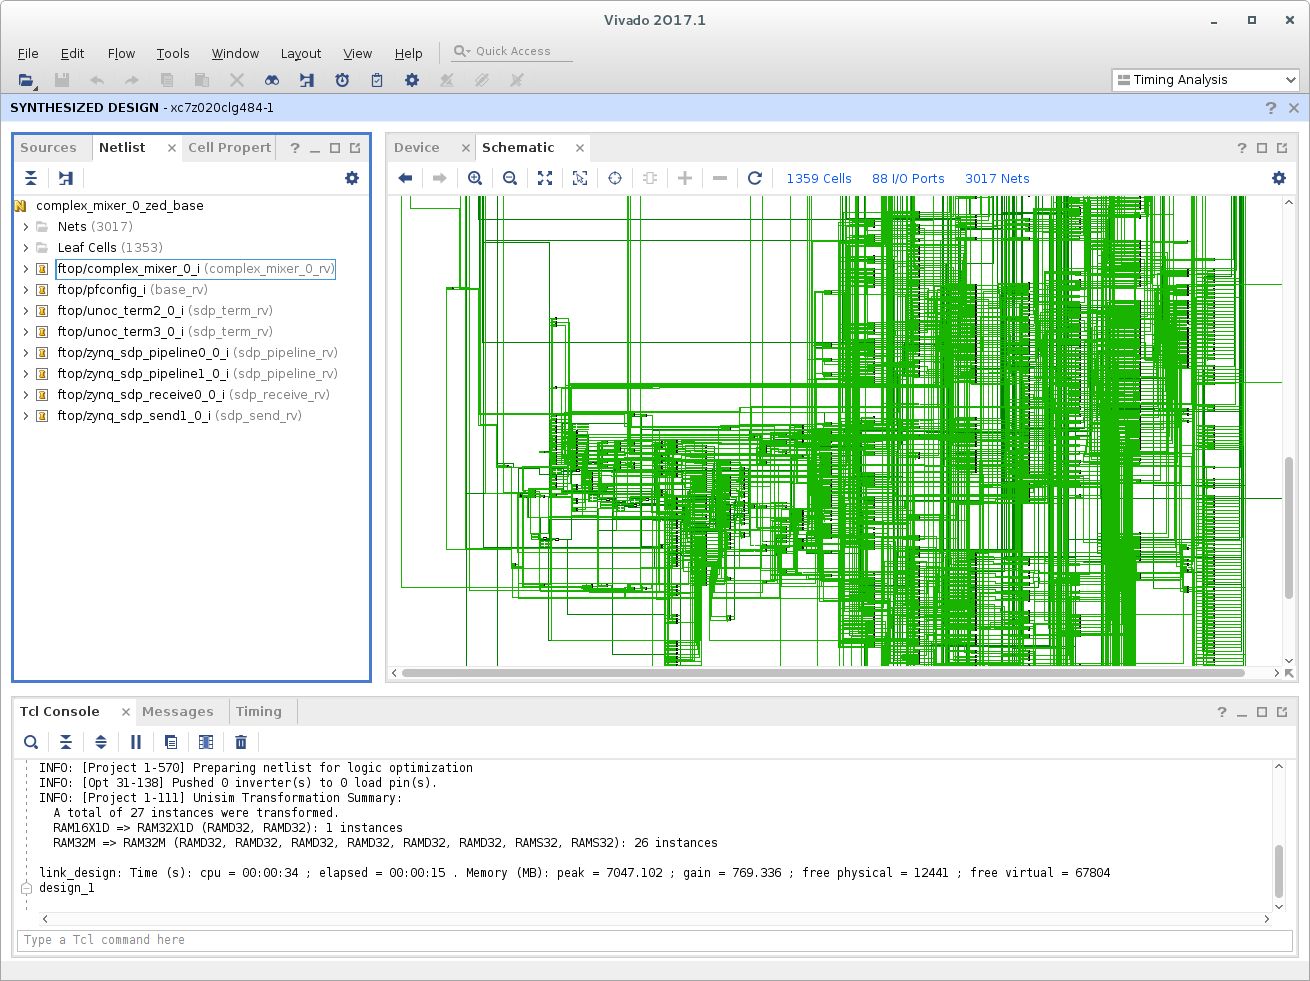
\includegraphics[scale=0.4]{figures/xilinx_vivado_netlist}}
	\caption{Xilinx Vivado Netlist}
\end{figure}

Another option for viewing EDIF netlists in Vivado involves creating a Post-Synthesis project and including the netlist as a source file. You can then ``Open Synthesized Design'' to view the netlist in the GUI.
\subsection{Project File}
To open up a Vivado project at any level, run:\newline
\code{vivado target-<tgt>/<asset-name>.xpr}\newline

Because the framework runs compilation in Non-Project Mode, the source files and synthesis results will not be opened side-by-side.
\begin{figure}[H]
	\centerline{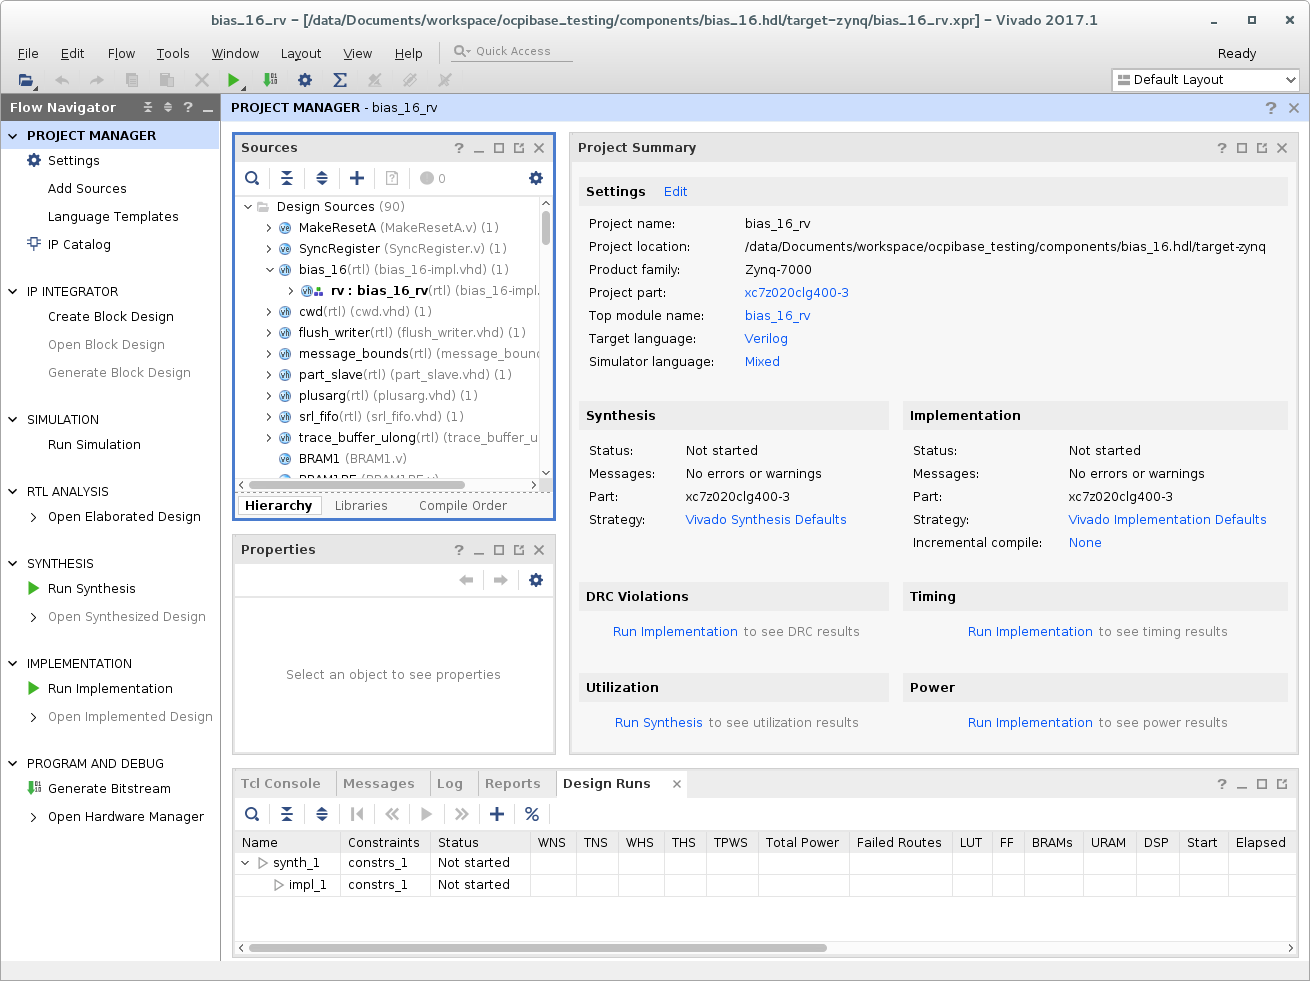
\includegraphics[scale=0.4]{figures/xilinx_vivado_project_view}}
	\caption{Xilinx Vivado Project}
\end{figure}
However, after a project file is opened in the GUI, synthesis can be rerun in Project Mode. The synthesized design can then be opened, and the netlist and source can be viewed together.
\begin{figure}[H]
	\centerline{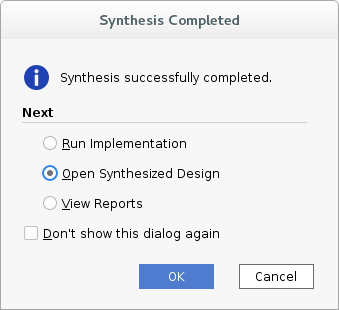
\includegraphics[scale=0.6]{figures/xilinx_vivado_open_synth}}
	\caption{Xilinx Vivado Open Synthesized Design}
\end{figure}
After this, netlists and sources can be viewed together.
\begin{figure}[H]
	\centerline{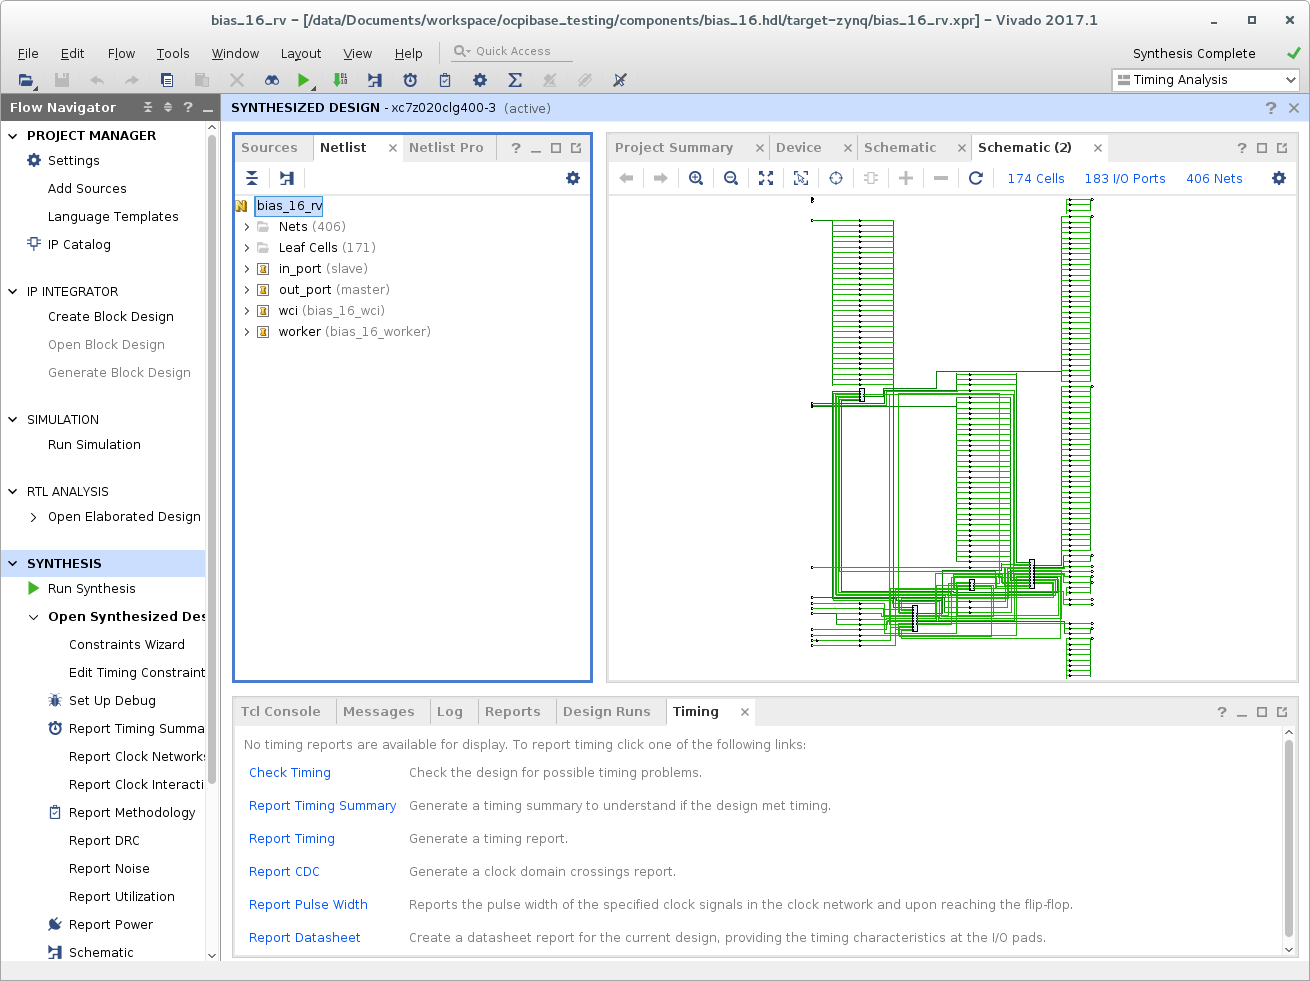
\includegraphics[scale=0.4]{figures/xilinx_vivado_netlist_view}}
	\caption{Xilinx Vivado Netlist View}
\end{figure}
At this point, you can right click on elements of the netlist and ``Go To Source''.\newline

The various stages of implementation also generate project files. These project files can be opened, and implementation can be run in Project-Mode via the Vivado GUI. The other option for viewing implementation results is to open an implementation-stage's checkpoint as described in \ref{dcp}.

\subsection{Implementation Design Checkpoint}
\label{dcp}
To open up a Vivado Design Checkpoint resulting from any post-synthesis implementation stage, run:\newline
\code{vivado <path-to-OCPI-container-dir>/target-<tgt>/<OCPI-container-name>-<stage>.dcp}\newline
\begin{figure}[H]
	\centerline{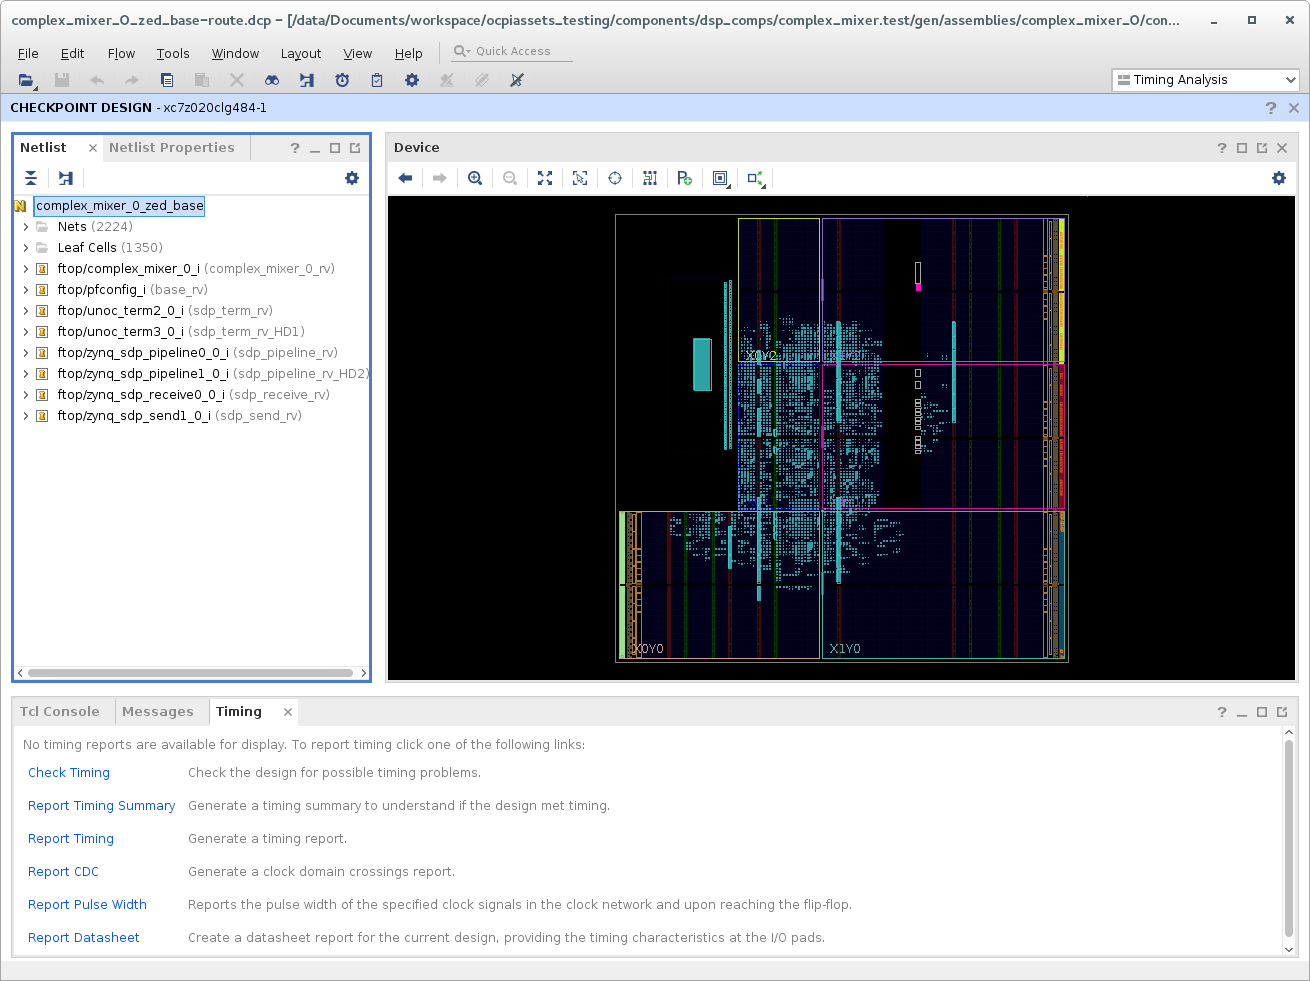
\includegraphics[scale=0.4]{figures/xilinx_vivado_post_route_dcp}}
	\caption{Xilinx Vivado Post-Route Design Checkpoint}
\end{figure}

\subsection{Interactive Timing Report}
To open up an interactive timing report (result of timing stage of implementation):
\begin{enumerate}
\item Open up the Design Checkpoint for the route stage (shown in \ref{dcp}).
\item Open the interactive timing report:
\subitem File $\rightarrow$ Open Interactive Report $\rightarrow$ \code{<container-name>-timing.rpx}
\end{enumerate}
\begin{figure}[H]
	\centerline{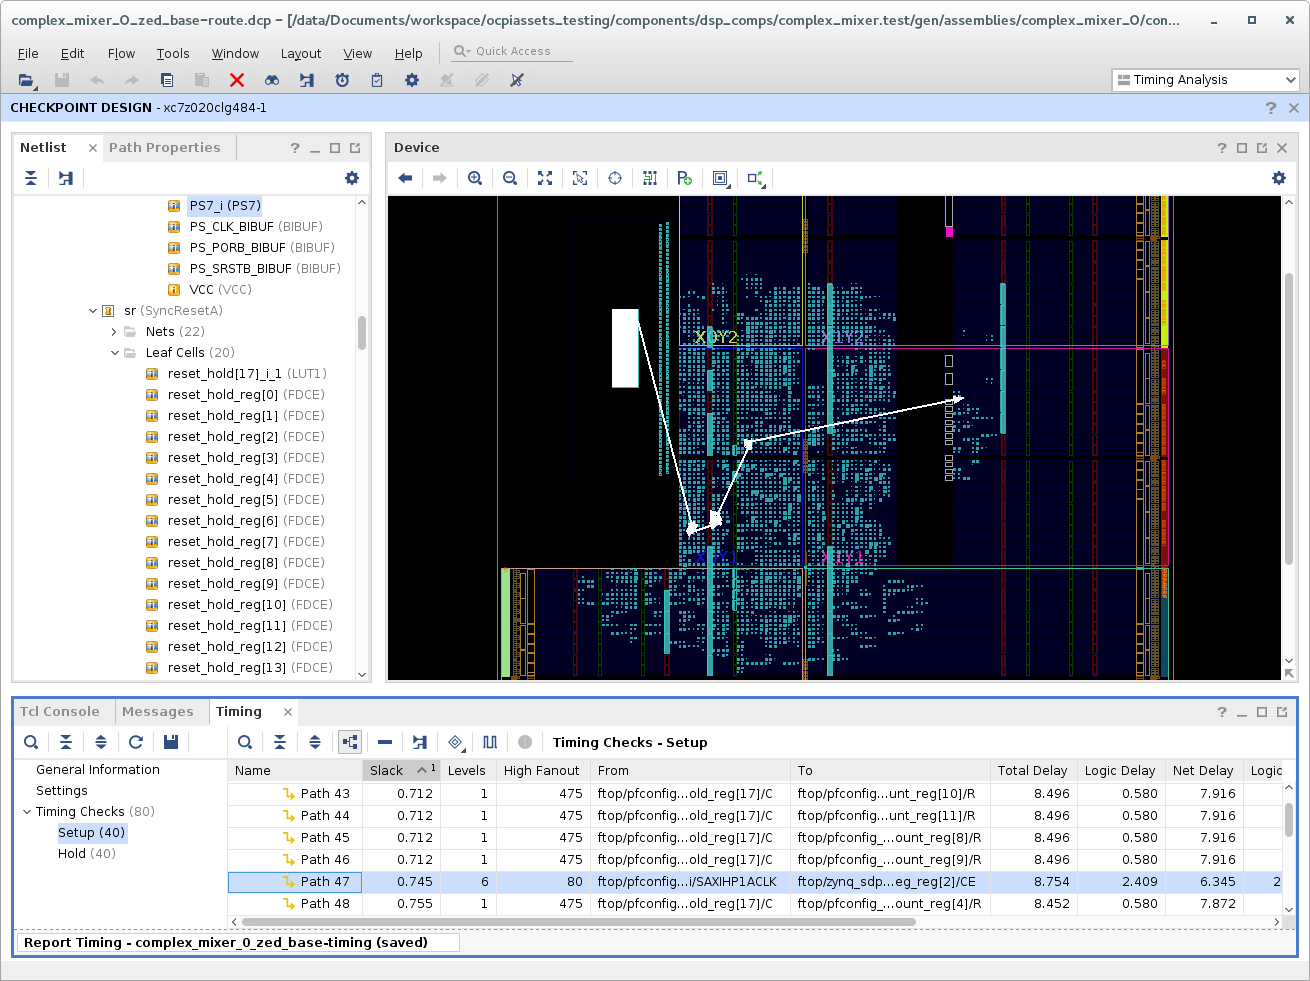
\includegraphics[scale=0.4]{figures/xilinx_vivado_interactive_timing_report}}
	\caption{Xilinx Vivado Interactive Timing Report}
\end{figure}

\subsection{Elaborated XSIM design}
To open up the results of XSIM's \code{xelab}:\newline
\code{xsim <path-to-OCPI-container-dir>/target-<tgt>/<OCPI-container-name>}\newline
\begin{figure}[H]
	\centerline{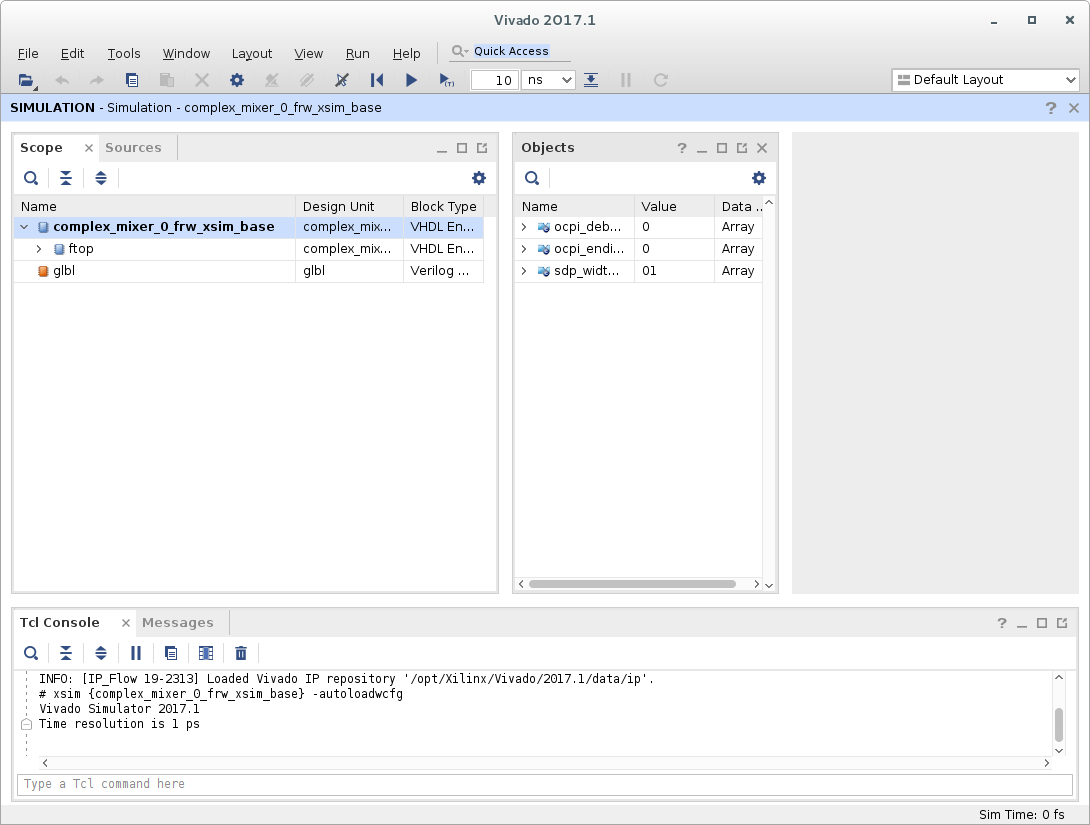
\includegraphics[scale=0.4]{figures/xilinx_xsim_elaborated_design}}
	\caption{Xilinx Vivado Simulator Elaborated Design}
\end{figure}

\subsection{Open XSIM Wave Database}
As with any other simulator, you can run:\newline
\code{ocpiview <simulations-directory>}\newline
For example, for the complex\_mixer.test Unit Test, after running case00.00 with \code{ocpidev}'s \code{--keep-simulations} option (or Make's \code{KeepSimulations=1}) set, you can run:\newline
\code{ocpiview run/xsim/case00.00.complex\_mixer.hdl.simulation}
\begin{figure}[H]
	\centerline{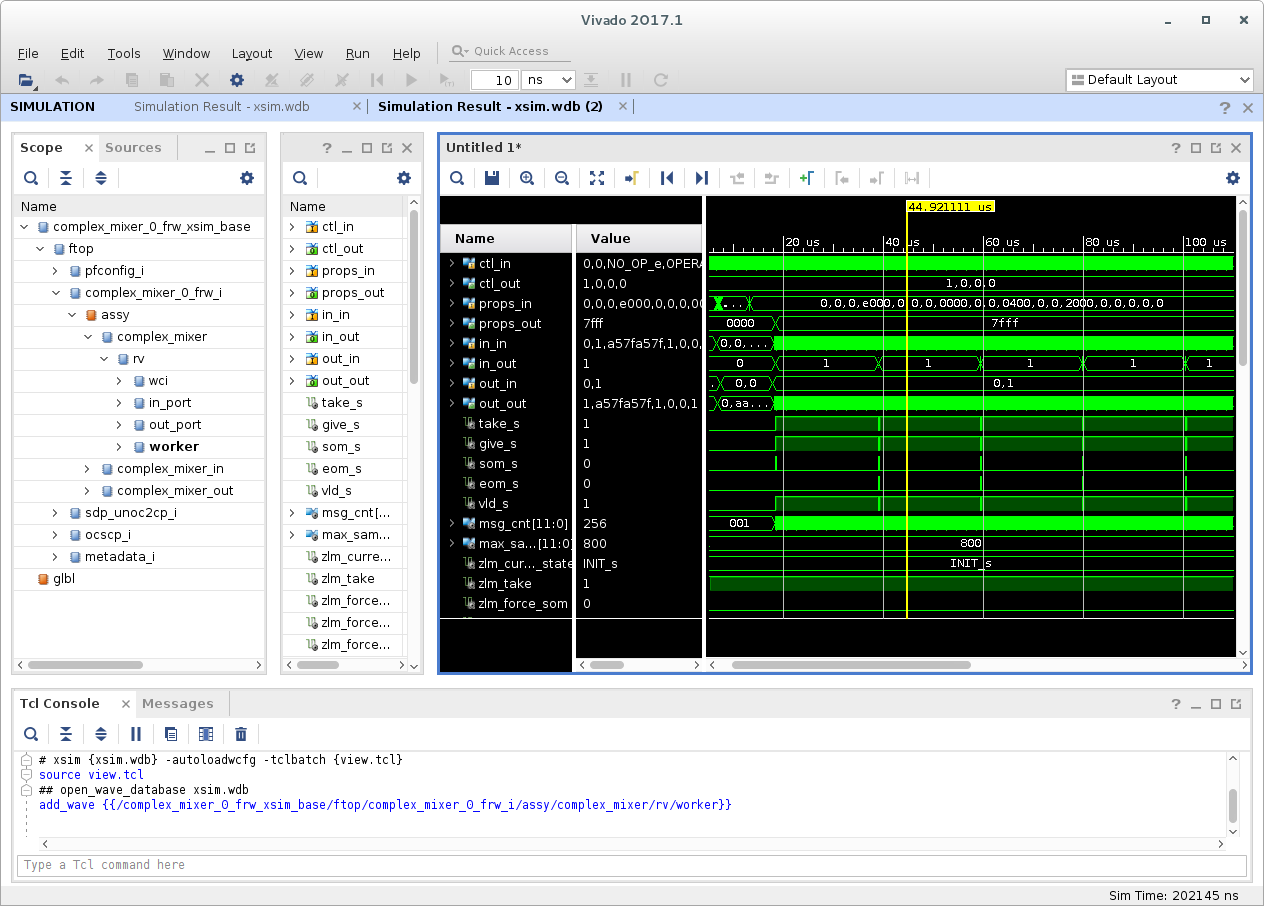
\includegraphics[scale=0.4]{figures/xilinx_xsim_ocpiview}}
	\caption{Xilinx Vivado Simulator Wave Database}
\end{figure}


\section{OpenCPI Output Files for Vivado}
\begin{itemize}
\item \code{.jou}: Vivado journal file
\item \code{.jou.bak}: Backup of the previously generated Vivado journal file
\item \code{<asset-name>-vivado.out}: OpenCPI \textit{and} Vivado output for synthesis of an asset
\item \code{<impl-stage>.out}: OpenCPI \textit{and} Vivado output for a stage of implementation
\item \code{.xpr}: Every stage of compilation for every OpenCPI asset results in a Vivado project file. This project file can be opened in Vivado to observe the source files associated with that stage.
\item \code{.edf}: Vivado's netlist format. This is the artifact of building any OpenCPI asset except primitive libraries.
\item \code{.dcp}: After the container is synthesized, implementation begins. From then on, DCP (Vivado's Design Checkpoint) files are used as the result of each implementation stage.
\item \code{.rpx}: Vivado's Interactive Timing Report. This file is generated as a result of the \code{timing} stage which is run after \code{route}.
\item \code{.libs}, \code{.sources}, \code{.cores}: The OpenCPI files used to store information regarding the libraries, sources, and cores that an asset depends on
\item \code{*.hw, *.ip\_user\_files, *.cache} directories: Various directories generated by Vivado when creating a project or running synthesis/implementation stages
\end{itemize}
\section{OpenCPI Output Files for XSIM}
\begin{itemize}
\item \code{.log}: XSIM log file for \code{xelab}, \code{xvhdl}, and \code{xvlog} commands
\item \code{.vdb}: Output of XSIM's source parser
\item \code{xsim.dir}: Files generated by XSIM during setup and elaboration
\item \code{.pb}: Message information for Vivado's ``Messages'' window
\end{itemize}
\end{flushleft}
\end{document}
